\documentclass{beamer}
% \usepackage[utf8]{inputenc}
\usepackage[T1]{fontenc}
\usetheme{CambridgeUS}
\usecolortheme{dove}
\usefonttheme{serif}

\usepackage[english]{babel}
% \usepackage[english, polish]{babel}

\usepackage{listings}
\usepackage{siunitx}
\usepackage{pifont}
\usepackage{amsmath,amssymb,amsfonts}
\usepackage{graphicx}
\usepackage{float}
\usepackage{xcolor}
\usepackage{setspace}

\newcommand{\todo}[1]{\textcolor{red}{TODO: #1}}

\newcommand{\imagesource}[1]{
    \begin{spacing}{0.5}
        \texttt{\textit{ \tiny{source: #1}}}
    \end{spacing}
}




\title{GSI Green Cube}
    \subtitle{\textit{High-Performance Computing in Nuclear Physics Research}}
\author{Tobiasz Fic}
\date{19 May 2024}

\begin{document}

\begin{frame}
    \maketitle
\end{frame}

\begin{frame}{GSI and FAIR}
    \begin{columns}
        \begin{column}{0.5\textwidth}
            \begin{figure}
                \centering
                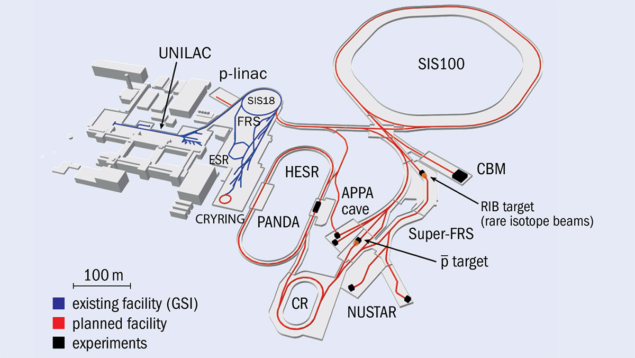
\includegraphics[width=\textwidth]{images/fair_sis100_diagram.jpg}
            \end{figure}
        \end{column}
        \begin{column}{0.5\textwidth}
            \begin{itemize}
                \item GSI (Gesellschaft für Schwerionenforschung) Helmholtzzentrum für Schwerionenforschung is a nuclear research facility in Darmstadt, Germany.
                \item The FAIR particle accelerator  facility is under construction (due 2027).
            \end{itemize}
        \end{column}
    \end{columns}
\end{frame}


\begin{frame}{Need for High-Performance Computing}
    \begin{columns}
        \begin{column}{0.5\textwidth}
            \begin{itemize}
                \item The rising complexity of nuclear physics experiments requires more computational power.
                \item Example: the CBM experiment will have an interaction rate of \SI{10}{\mega\hertz}.
            \end{itemize}
        \end{column}
        \begin{column}{0.5\textwidth}
            \begin{figure}
                \centering
                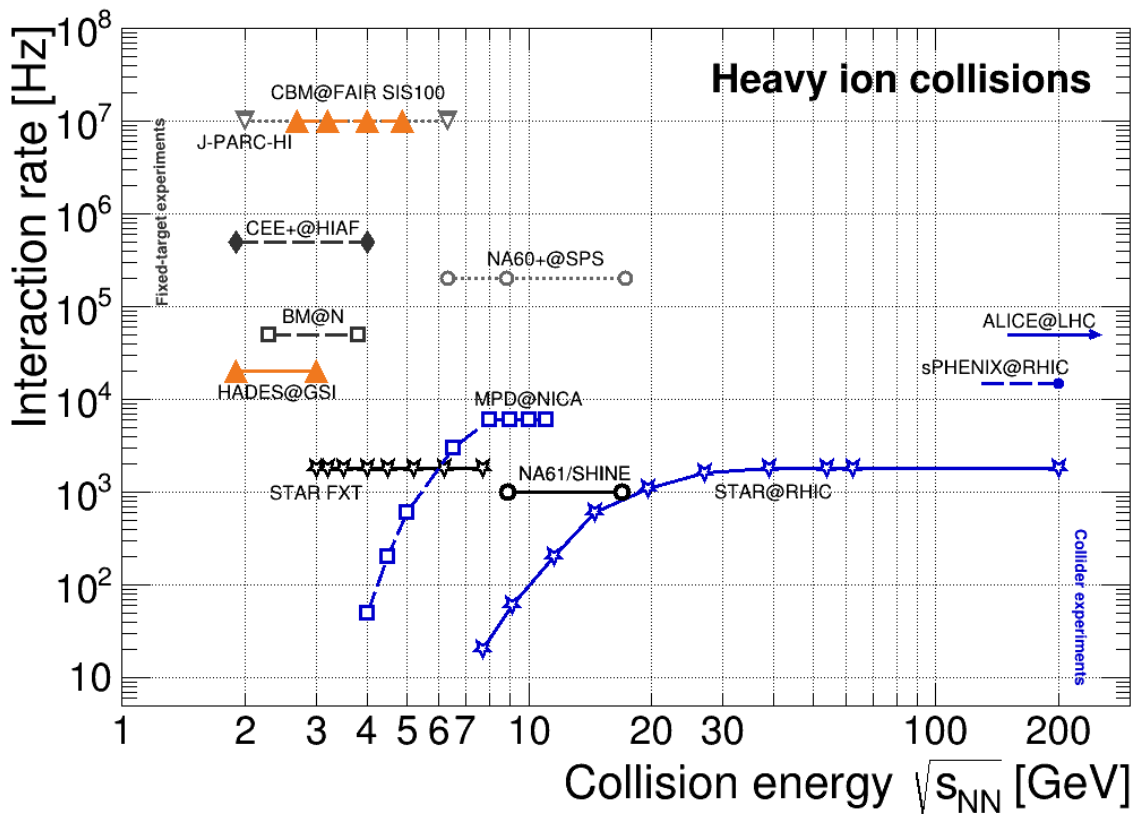
\includegraphics[width=\textwidth]{images/galatyuk_map_of_experiments.png}
                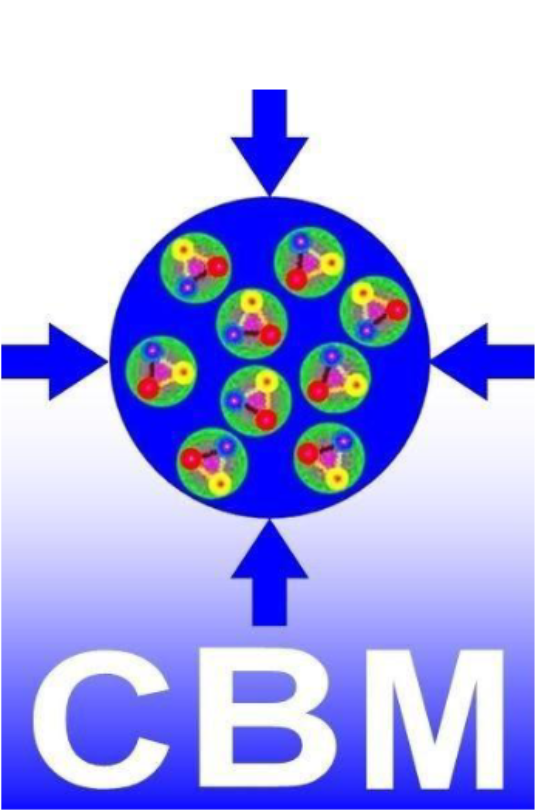
\includegraphics[width=0.2\textwidth]{images/cbm_logo.png}
                \imagesource{CBM Collaboration, EPJA 53 3 (2017) 60 T. Galatyuk, NPA982 (2019), update (2021)}
            \end{figure}
        \end{column}
    \end{columns}
\end{frame}

\begin{frame}{Green Cube Data Center}
    \begin{columns}
        \begin{column}{0.5\textwidth}
            \begin{figure}
                \centering
                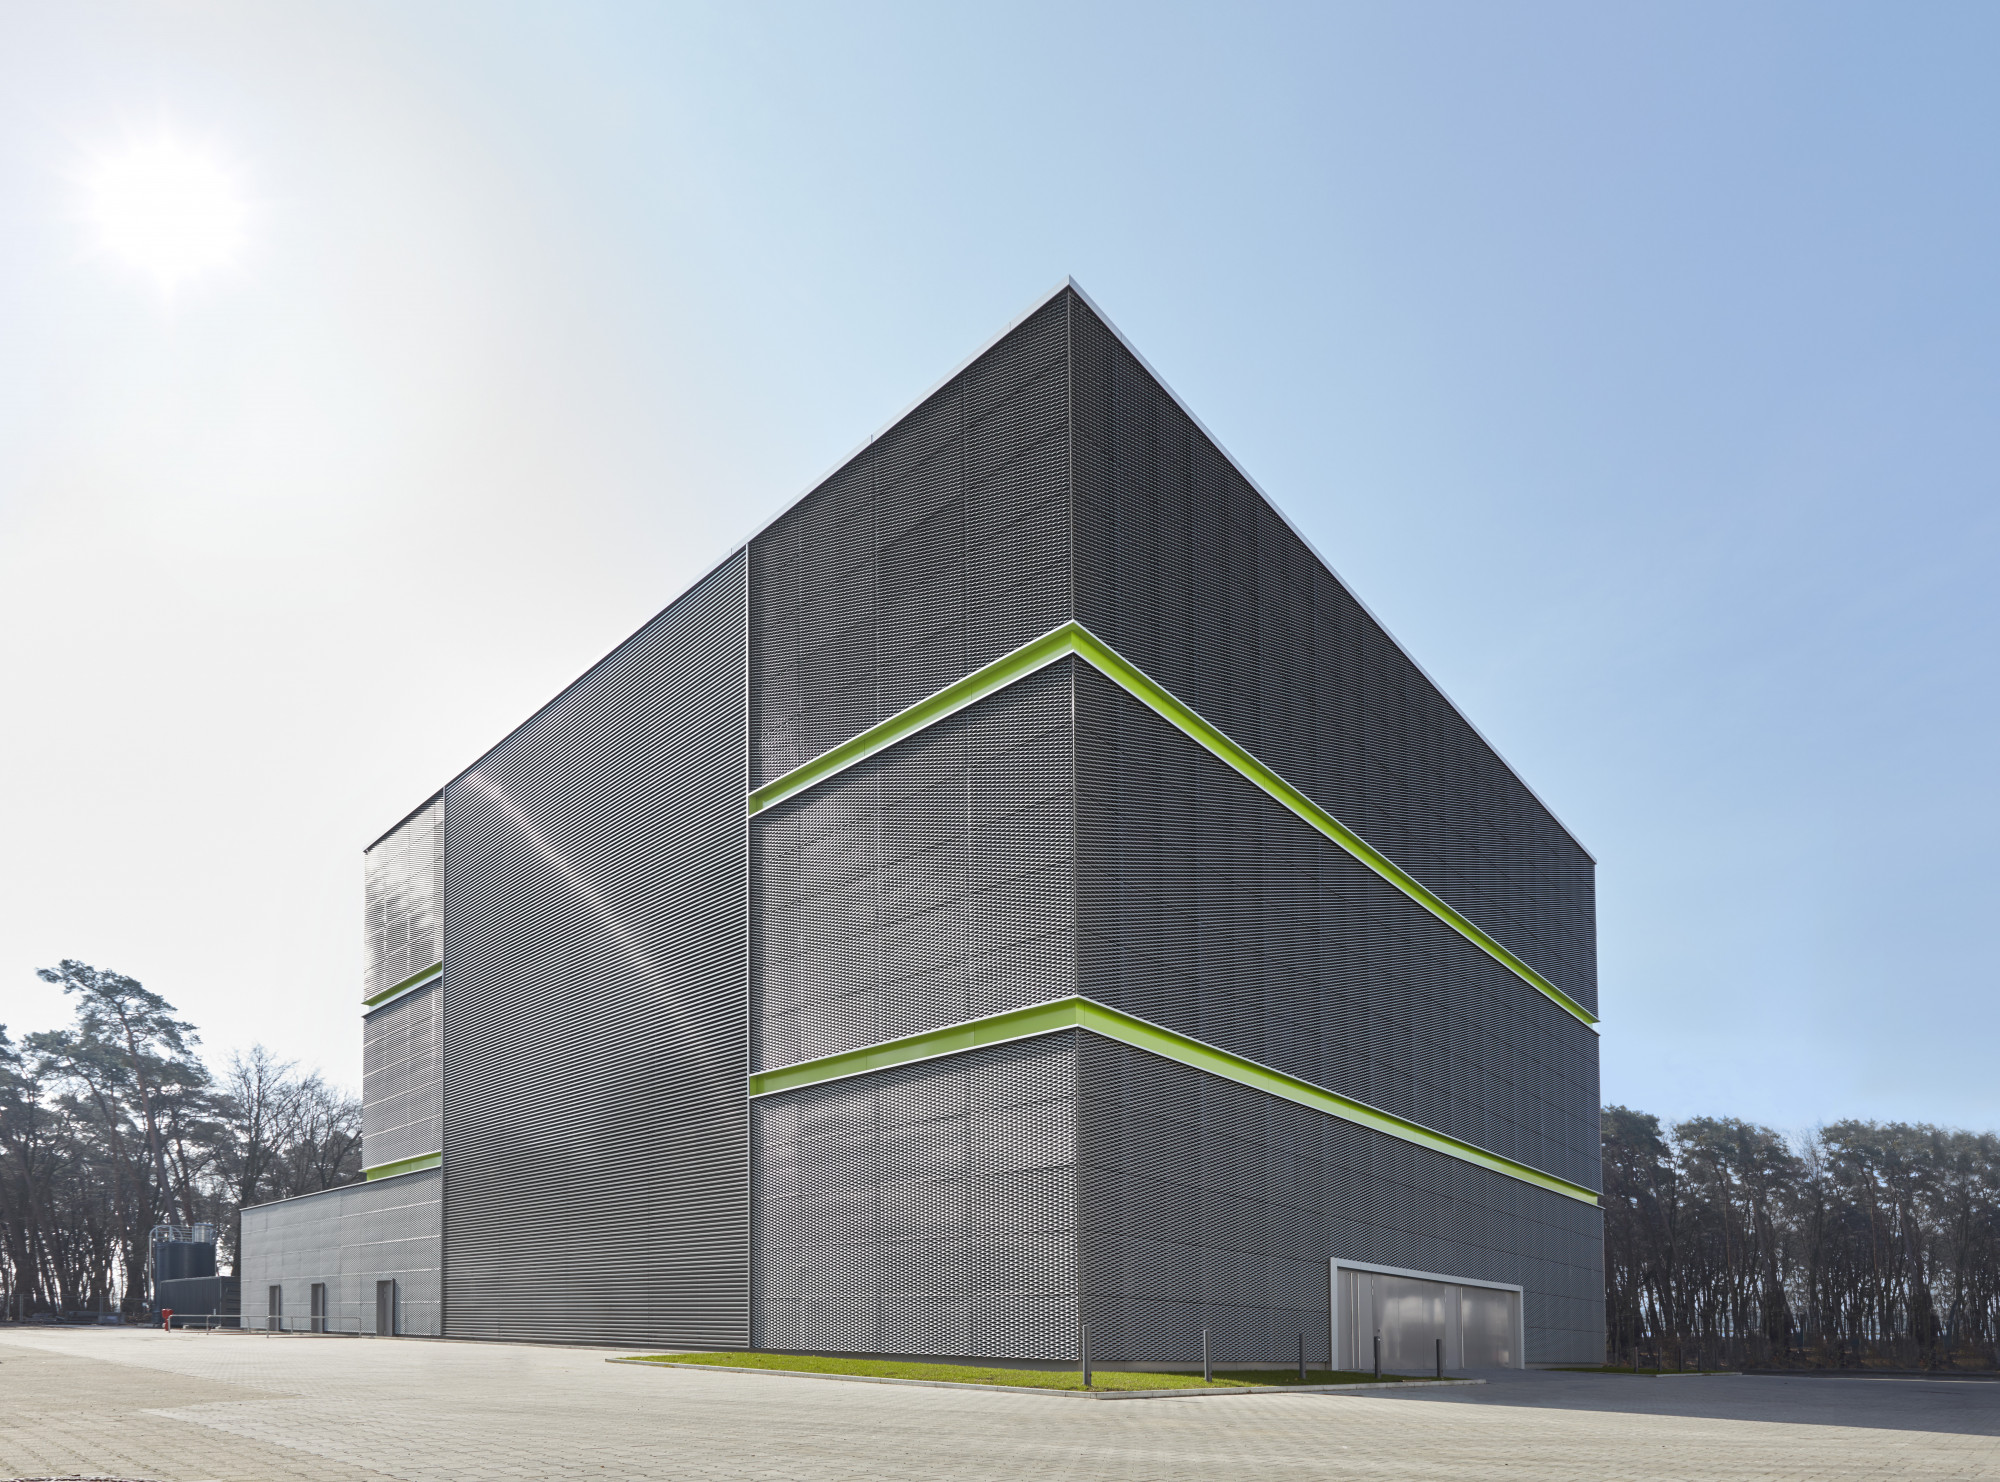
\includegraphics[width=\textwidth]{images/gsi_green_cube.jpg}
                \imagesource{https://ttsp-hwp.de/en/project/gsi/}
            \end{figure}
        \end{column}
        \begin{column}{0.5\textwidth}
            \begin{itemize}
                \item The Green Cube was built in 2015 as a solution to the growing computational needs of GSI (and in the future, FAIR).
                \item The investment totaled \num{12} million euros in construction costs and \num{21} million euros overall.
            \end{itemize}
        \end{column}
    \end{columns}
\end{frame}

\begin{frame}{Green Cube: Inside}
    \begin{columns}
        \begin{column}{0.5\textwidth}
            \begin{itemize}
                \item Inside the temperature is kept at around 15 degrees, even in the summer
                \item During the winter the heat recuperated from the working nodes is used to heat up the canteen nextdoor
            \end{itemize}
        \end{column}
        \begin{column}{0.5\textwidth}
            \begin{figure}
                \centering
                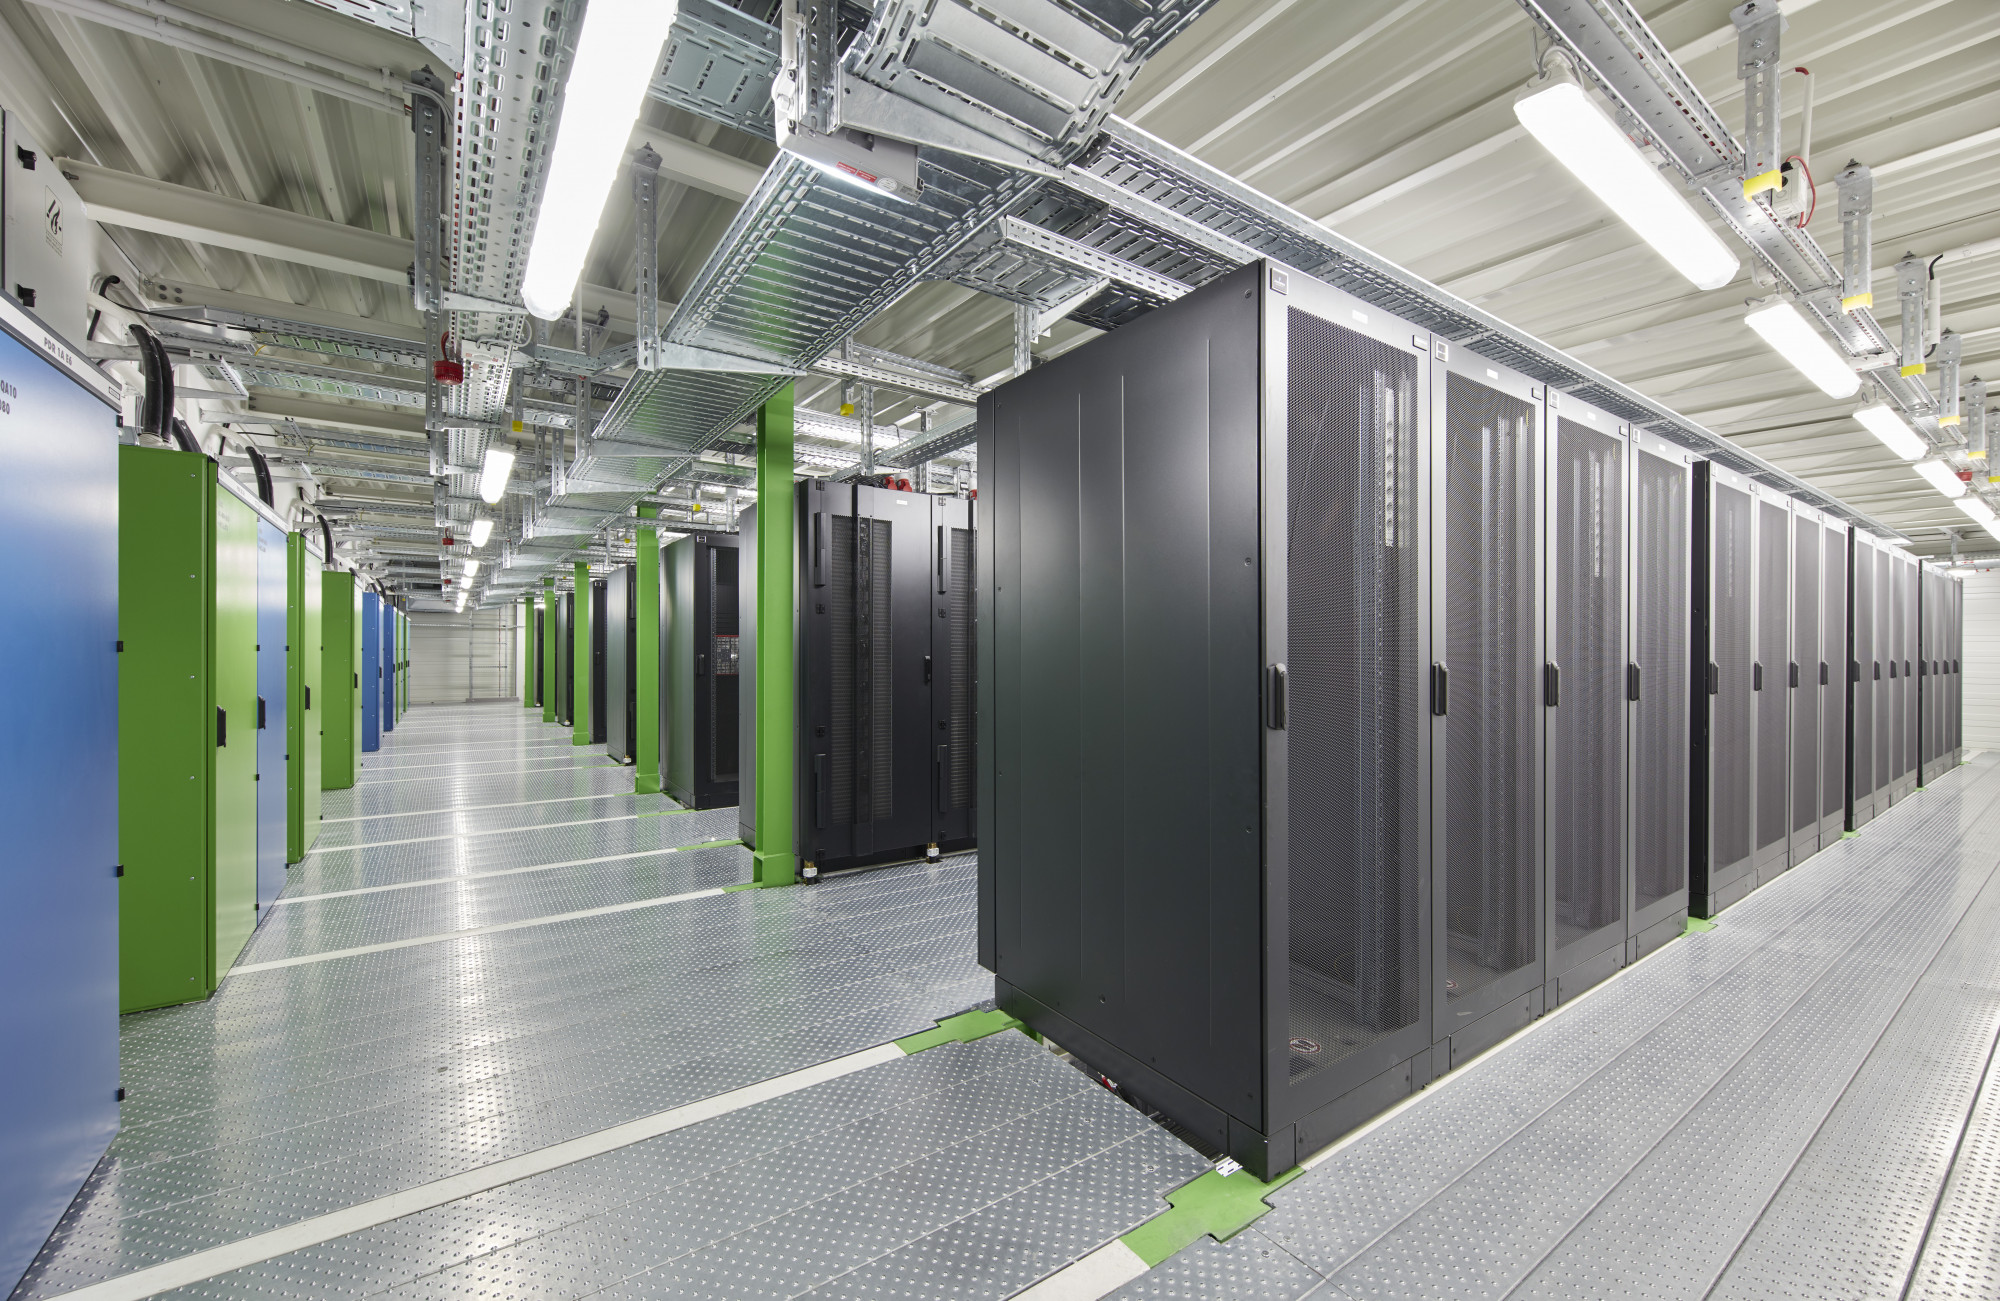
\includegraphics[width=\textwidth]{images/gsi_green_cube_inside.jpg}
                \imagesource{https://ttsp-hwp.de/en/project/gsi/}
            \end{figure}
        \end{column}
    \end{columns}
\end{frame}

% overall specs
\begin{frame}{Green Cube: Overall Specs}
    \begin{columns}
        \begin{column}{0.5\textwidth}
            \begin{itemize}
                \item size: 27 \si{\meter} x 30 \si{\meter} x height 22 \si{\meter} (6 levels)
                \item 12 \si{\mega\watt} cooling capability
                \item 600 nodes, on average 90 cores per node
                \item 400 GPUs
            \end{itemize}
        \end{column}
        \begin{column}{0.5\textwidth}
            \begin{itemize}
                \item Maximum number of racks: 768 2.2 \si{\meter} racks
                \item 60 petabytes of storage, will be expanded to 250 petabytes for FAIR
            \end{itemize}
        \end{column}
    \end{columns}
\end{frame}


\begin{frame}{Software: \textit{Singularity} containers}
    \begin{columns}
        \begin{column}{0.4\textwidth}
            \begin{figure}
                \centering
                
\includegraphics[width=\textwidth]{images/singularity_logo.png}
                \imagesource{https://docs.sylabs.io/}
            \end{figure}
        \end{column}
        \begin{column}{0.6\textwidth}
            \begin{itemize}
                \item Singularity containers are used to encapsulate software environments. (like docker)
                \item Each time a job is launched, or a user signs in, a new container is created.
            \end{itemize}
        \end{column}
    \end{columns}
\end{frame}

% lustre
\begin{frame}{Software: \textit{Lustre} File System}
    \begin{columns}
        \begin{column}{0.6\textwidth}
            \begin{itemize}
                \item High-performance distributed file system.
                \item Open-source, POSIX-compliant.
                \item Used in many supercomputers and data centers.
                \item Scalable to thousands of devices.
            \end{itemize}
        \end{column}
        \begin{column}{0.4\textwidth}
            \begin{figure}
                \centering
                
\includegraphics[width=\textwidth]{images/lustre_logo.png}
                \imagesource{https://www.lustre.org/}
            \end{figure}
        \end{column}
    \end{columns}
\end{frame}

\begin{frame}[fragile]{Lustre: Mounting the File System Remotely}
    \begin{columns}
        \begin{column}{0.4\textwidth}
            \begin{figure}
                \centering
                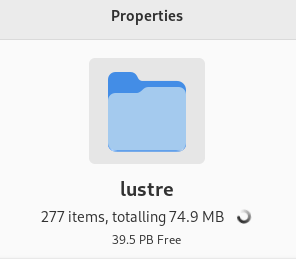
\includegraphics[width=\textwidth]{images/lustre_petabytes.png}
            \end{figure}
        \end{column}
        \begin{column}{0.6\textwidth}
            In a file, such as \texttt{mount.sh}:
            \begin{lstlisting}[language=bash]
mnt='/tmp/lustre/'
mkdir -p $mnt
sshfs -o ProxyJump=lxpool.gsi.de tfic@lustre.hpc.gsi.de:/lustre $mnt
            \end{lstlisting}
            then, to mount the file system:
            \begin{lstlisting}[language=bash]
bash mount.sh
            \end{lstlisting}
            to unmount:
            \begin{lstlisting}[language=bash]
fusermount -u $mnt
            \end{lstlisting}
        \end{column}
    \end{columns}
\end{frame}

% working nodes

% slurm workload manager
\begin{frame}{Software: \textit{SLURM} Workload Manager}
    \begin{columns}
        \begin{column}{0.6\textwidth}
            \begin{itemize}
                \item Workload manager for Linux clusters.
                \item Open-source.
                \item Used in many supercomputers and data centers.
                \item Scalable to thousands of devices.
                \item Easy to use: \texttt{sbatch}, \texttt{srun}, \texttt{squeue}, \texttt{sinfo}.
                      Work gets delegated to nodes automatically through bash scripts or commands.
            \end{itemize}
        \end{column}
        \begin{column}{0.4\textwidth}
            \begin{figure}
                \centering
                
\includegraphics[width=0.5\textwidth]{images/slurm_logo.png}
                \imagesource{https://slurm.schedmd.com/}
            \end{figure}
        \end{column}
    \end{columns}
\end{frame}

\begin{frame}[fragile]{SLURM: Example Job Script}
    \begin{columns}
        \begin{column}{0.4\textwidth}
            \begin{figure}
                \centering
                
\includegraphics[width=0.5\textwidth]{images/slurm_logo.png}
            \end{figure}
        \end{column}
        \begin{column}{0.6\textwidth}
            In a file, such as \texttt{job.sh}:
            \begin{lstlisting}[language=bash]
#!/bin/bash
#SBATCH --output %j_%N.out
hostname ; sleep ${1:-30}
            \end{lstlisting}
            then, to launch the script as a job:
            \begin{lstlisting}[language=bash]
sbatch job.sh
            \end{lstlisting}
            to check job status:
            \begin{lstlisting}[language=bash]
squeue -u $USER 
            \end{lstlisting}
            to cancel a job:
            \begin{lstlisting}[language=bash]
scancel <job_id>
            \end{lstlisting}
        \end{column}
    \end{columns}
\end{frame}

\begin{frame}{Software: CVMFS Software distribution}
    \begin{columns}
        \begin{column}{0.6\textwidth}
            \begin{itemize}
                \item CernVM File System.
                \item Some of the programs used for simulation and analysis take very long to compile,
                      so they are cached and distributed through CVMFS which is interfaced as a directory of compiled
                      versions of the programs on Lustre.
            \end{itemize}
        \end{column}
        \begin{column}{0.4\textwidth}
            \begin{figure}
                \centering
                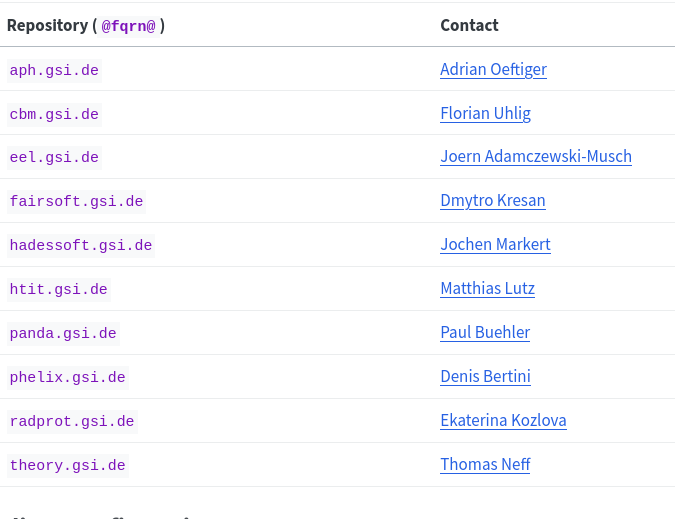
\includegraphics[width=\textwidth]{images/cvmfs_list.png}
                \imagesource{https://hpc.gsi.de/virgo/user-guide/
                    overview/cvmfs.html}
            \end{figure}
        \end{column}
    \end{columns}

\end{frame}

\begin{frame}[fragile]{Green Cube at work: CBMRoot (on top of ROOT/GEANT4)}
    \begin{columns}
        \begin{column}{0.6\textwidth}
            \begin{figure}
                \centering
                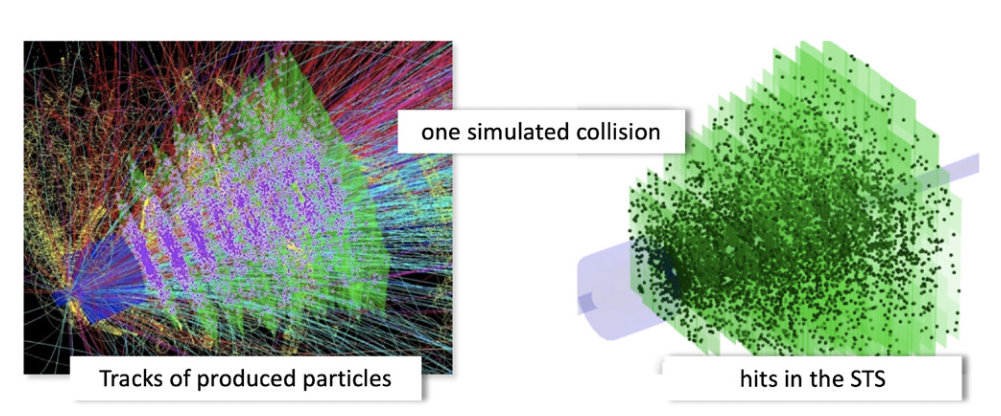
\includegraphics[width=\textwidth]{images/sts_reco.png}
                \imagesource{https://doi.org/10.1051/epjconf/202022601004}
            \end{figure}
        \end{column}
        \begin{column}{0.4\textwidth}
            \begin{itemize}
                \item The CBMRoot framework is built on top of GEANT4. It is used to simulate the passage of particles
                      through the CBM experiment's future detectors.
                \item The volume of data generated by these simulations is in the terabytes
            \end{itemize}
        \end{column}
    \end{columns}
\end{frame}

\begin{frame}[fragile]{Green Cube at work: HadesSoft (on top of ROOT)}
    \begin{columns}
        \begin{column}{0.4\textwidth}
            \begin{itemize}
                \item The HADES (High Acceptance DiElectron Spectrometer) experiment uses the HadesSoft framework to analyze
                      collision data.
            \end{itemize}
        \end{column}
        \begin{column}{0.6\textwidth}
            \begin{figure}
                \centering
                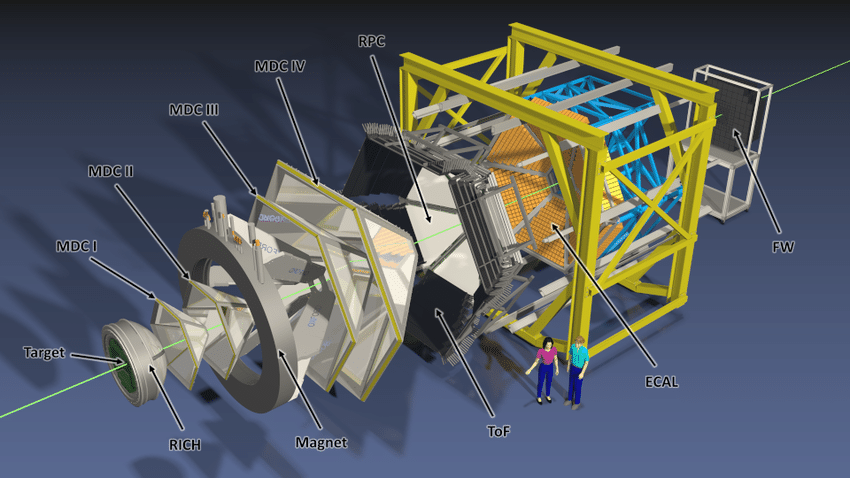
\includegraphics[width=\textwidth]{images/HADES_detectors.png}
                \imagesource{https://www.researchgate.net/publication/358337013/}
            \end{figure}
        \end{column}
    \end{columns}
\end{frame}

\begin{frame}{}
    \centering
    \Large{Questions?}
\end{frame}


\begin{frame}{}
    \centering
    \Large{Thank you for your attention}
\end{frame}



\end{document}
